\documentclass{standalone}
\usepackage{tikz}
\usetikzlibrary{shapes,arrows, positioning, calc, fit}
\tikzset{every node/.style={font=\sffamily}}
\begin{document}
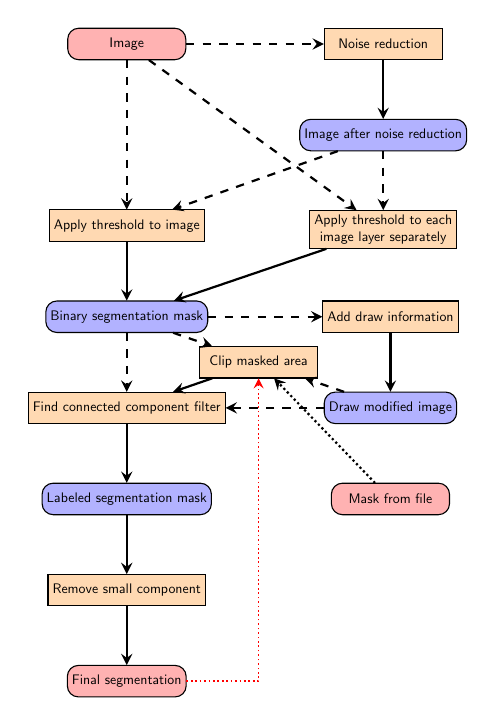
\begin{tikzpicture}[scale=0.5, node distance=1.5cm, transform shape]
  \tikzstyle{startstop} = [rectangle, rounded corners, minimum width=3cm, minimum height=.8cm,text centered, draw=black, fill=red!30]
  \tikzstyle{data} = [rectangle, rounded corners, minimum width=3cm, minimum height=.8cm,text centered, draw=black, fill=blue!30]
  \tikzstyle{process} = [rectangle, minimum width=3cm, minimum height=.8cm, align=center, draw=black, fill=orange!30]
  \tikzstyle{decision} = [diamond, minimum width=3cm, aspect=4, align=center, draw=black, fill=green!30]
  \tikzstyle{arrow} = [thick,->,>=stealth]
  \node (image) [startstop] {Image};
  \node (noise) [process, right=of image, xshift=2cm] {Noise reduction};
  \node (threshold) [process, below=of image, yshift=-2.3cm] {Apply threshold to image};
  \node (gaussimage) [data, below=of noise] {Image after noise reduction};
  \node (layerthreshold) [process, below=of gaussimage] {Apply threshold to each\\ image layer separately};
  \node (binmask) [data, below=of threshold] {Binary segmentation mask}; 
  \node (conn) [process, below=of binmask] {Find connected component filter};
  \node (bindraw) [data, right=of conn, xshift=1cm] {Draw modified image}; 
  \node (draw) [process, above=of bindraw] {Add draw information};
  \node (labeledmask) [data, below=of conn] {Labeled segmentation mask};
  \node (filter) [process, below=of labeledmask] {Remove small component};
  \node (final) [startstop, below=of filter] {Final segmentation};
  \node (mask) [process] at ($(conn)!0.5!(draw)$) {Clip masked area};
  \node (filemask) [startstop, below=of bindraw] {Mask from file};
  %\draw [arrow] (image) -- (threshold);
  \draw [arrow, dashed] (image) -- (threshold);
  \draw [arrow, dashed] (image) -- (noise);
  \draw [arrow] (noise) -- (gaussimage);
  \draw [arrow, dashed] (image) -- (layerthreshold);
  \draw [arrow, dashed] (gaussimage) -- (threshold);
  \draw [arrow, dashed] (gaussimage) -- (layerthreshold);
  \draw [arrow] (threshold) -- (binmask);
  \draw [arrow] (layerthreshold) -- (binmask);
  %\draw [arrow] (binmask) -- (conn); 
  \draw [arrow, dashed] (binmask) -- (conn);
  \draw [arrow, dashed] (binmask) -- (draw);
  \draw [arrow] (draw) -- (bindraw);
  %\draw [arrow] (bindraw) -- (conn);
  \draw [arrow, dashed] (bindraw) -- (conn);
  \draw [arrow, dashed] (bindraw) -- (mask);
  \draw [arrow, dashed] (binmask) -- (mask);
  \draw [arrow] (mask) -- (conn);
  \draw [arrow] (conn) -- (labeledmask);
  \draw [arrow] (labeledmask) -- (filter);
  \draw [arrow] (filter) -- (final);
  \draw [arrow, semithick, densely dotted, red] (final) -| (mask);
  \draw [arrow, densely dotted] (filemask) -- (mask);


\end{tikzpicture}
\end{document}
